%!TEX root=../report.tex

\section{Experiments and Evaluation}

Dynamic simulations are a method to support a hypothesis. I will analyze how game parameters influence the duration and how special cards impact the duration. The aim is to either confirm the \uno\ rules or to suggest modifications in order to achieve a better duration. I define the duration of a game as the number of rounds. The number of rounds is the number of turns devided by the number of players.  A assume a good duration for \uno\ is between 15 and 30 rounds. To convert the number of rounds to a duration in time, I assume that a turn takes five seconds on average. This value is derived from personal observations. 30 rounds of four players would result in a duration of ten minutes.
This kind of question are useful for game developers when they have to balance the game. For instance a game like \uno\ should not take to long, because it is mainly designed for kids.


\subsection{Impact of Special Cards}

The card deck of \uno\ includes some special cards. Special cards named special because they trigger an effect that is an unfair advantage or disadvantage. The special cards are \textit{wildcard} (chose new color), \textit{skip} (next player is skipped), \textit{plus2} (next player has to draw 2 cards or add a \textit{plus2} as well), \textit{wildcard plus4} (combination of wildcard and next player has to draw 4 cards). I analyzed multiple arrangements of special cards. Figure \ref{fig:impact-of-special-cards} shows a sorted scatter plot of the number of rounds. The plot reveals that adding the \textit{plus2} extends the game, while adding the \textit{wildcard} shortens the game. Adding all special cards rather extends the duration. With the aim of 15 to 30 rounds per game, the configuration with all special cards or only \textit{plus2}-cards works the best as shown in the histogram in figure \ref{fig:impact-of-special-cards-hist}.

\begin{figure}[h!]
  \caption{Simulation of 1000 Games of three players with seven hand cards and different configurations of the card deck}
  \centering
  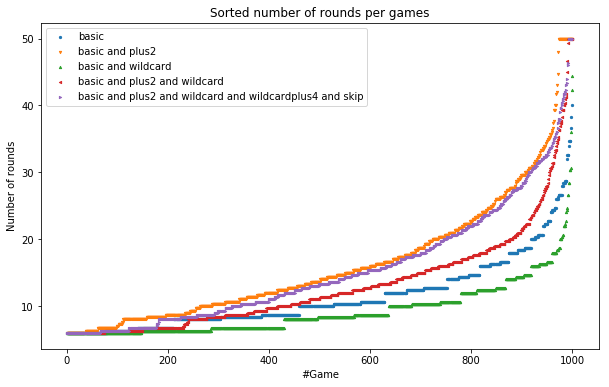
\includegraphics[width=0.9\textwidth]{impact-of-special-cards}
  \label{fig:impact-of-special-cards}
\end{figure}



\begin{figure}[h!]
  \caption{Histogram of simulation of 1000 Games of three players with seven hand cards and different configurations of the card deck. The bars indicate how many games ended after 0 to 15 rounds, 15 to 30 rounds, and more than 30 rounds.}
  \centering
  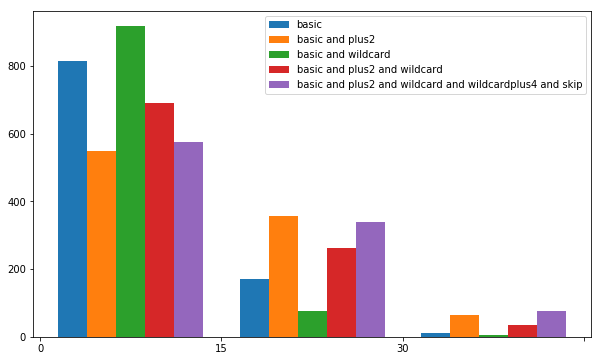
\includegraphics[width=0.9\textwidth]{impact-of-special-cards-histogram}
  \label{fig:impact-of-special-cards-hist}
\end{figure}


\subsection{Impact of Game Parameters}

The easiest parameter that can be tuned are number of hand cards according to the number of players. Therefore I simulated all combinations of two, three, four, five, seven and 10 players with three, five, seven and nine hand cards. The result is shown as boxplots in figure \ref{fig:boxplot-all-parameters}. An increase of players result in a decrease of rounds per game and in a smaller span of the result. More cards lead to an increase of rounds. Outliers of 100 or more rounds exist for all configurations up to five players. 100 is the maximum because the simulation stops after 100 rounds.



\begin{figure}[h!]
  \caption{Number of rounds to finish a game for a selection of two to ten players with three to 9 hand cards}
  \centering
  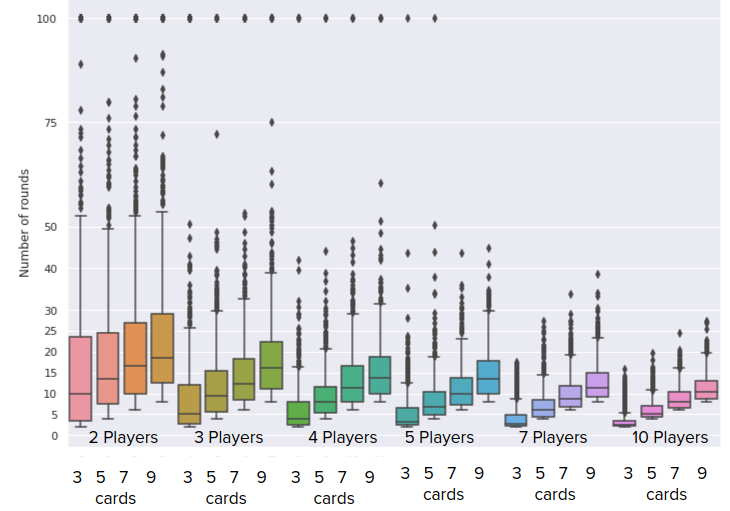
\includegraphics[width=0.9\textwidth]{boxplot-all-parameters}
  \label{fig:boxplot-all-parameters}
\end{figure}


%The histogram shows bars and percentage of games that end after 10-20 turns, 20-30 and so on. The more cards, the longer takes the game. The probability to finish after less than 20 turns is a bit to high with 3 or 5 cards in the beginning. 7 cards would mean that more than 50\% of the games would end after 20-40 turns.
%
%
%Second analysis the impact of the number of players. I simulate Uno with 7 cards per player and 2-6 players per game. The histograms show the percentage of games that end with 10 to 20 turns, or 20 to 30 turns and so on. The last interval is from 80 to 150. You can see that most games end after 30-40 turns. And more player automatically leads to more turns, thats why I normalized the distribution by the number of players. Et voila, with 6 players it is very likely that the game ends in less than 20 rounds while with two players games can be very long. So 7 cards seems also be ok from this perspective, but maybe it’s worth to think about a 2-player version and name it Uno - Das Duell.
%
%
%\begin{figure}[h!]
%  \caption{\note{number of turns to finish the game}}
%  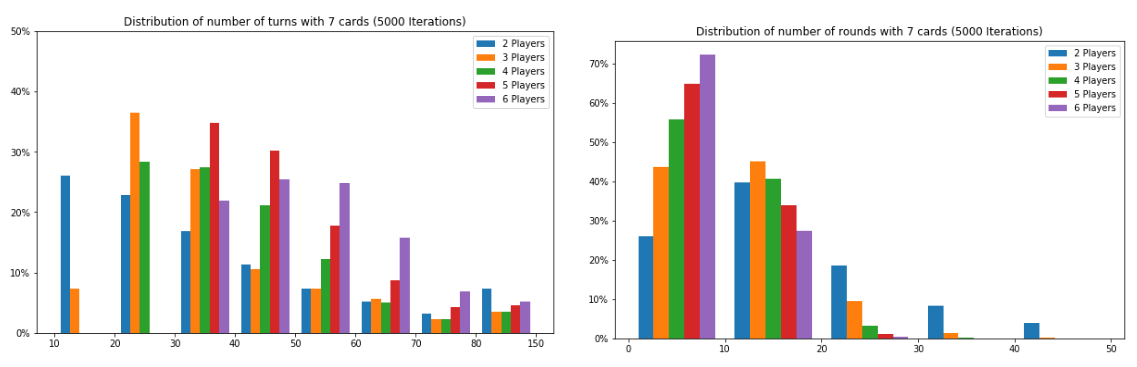
\includegraphics[width=0.9\textwidth]{histogram-players}
%\end{figure}
